\section{Sound from Musical Instruments}
Musical instruments also produce sound through a vibrating object inside them. In a guitar or veena, the strings vibrate. In a drum or a parai, the stretched membrane vibrates. In a Nadaswaram, flute, or a whistle, the air column inside the tube vibrates.
\begin{marginfigure}[-25\baselineskip]
  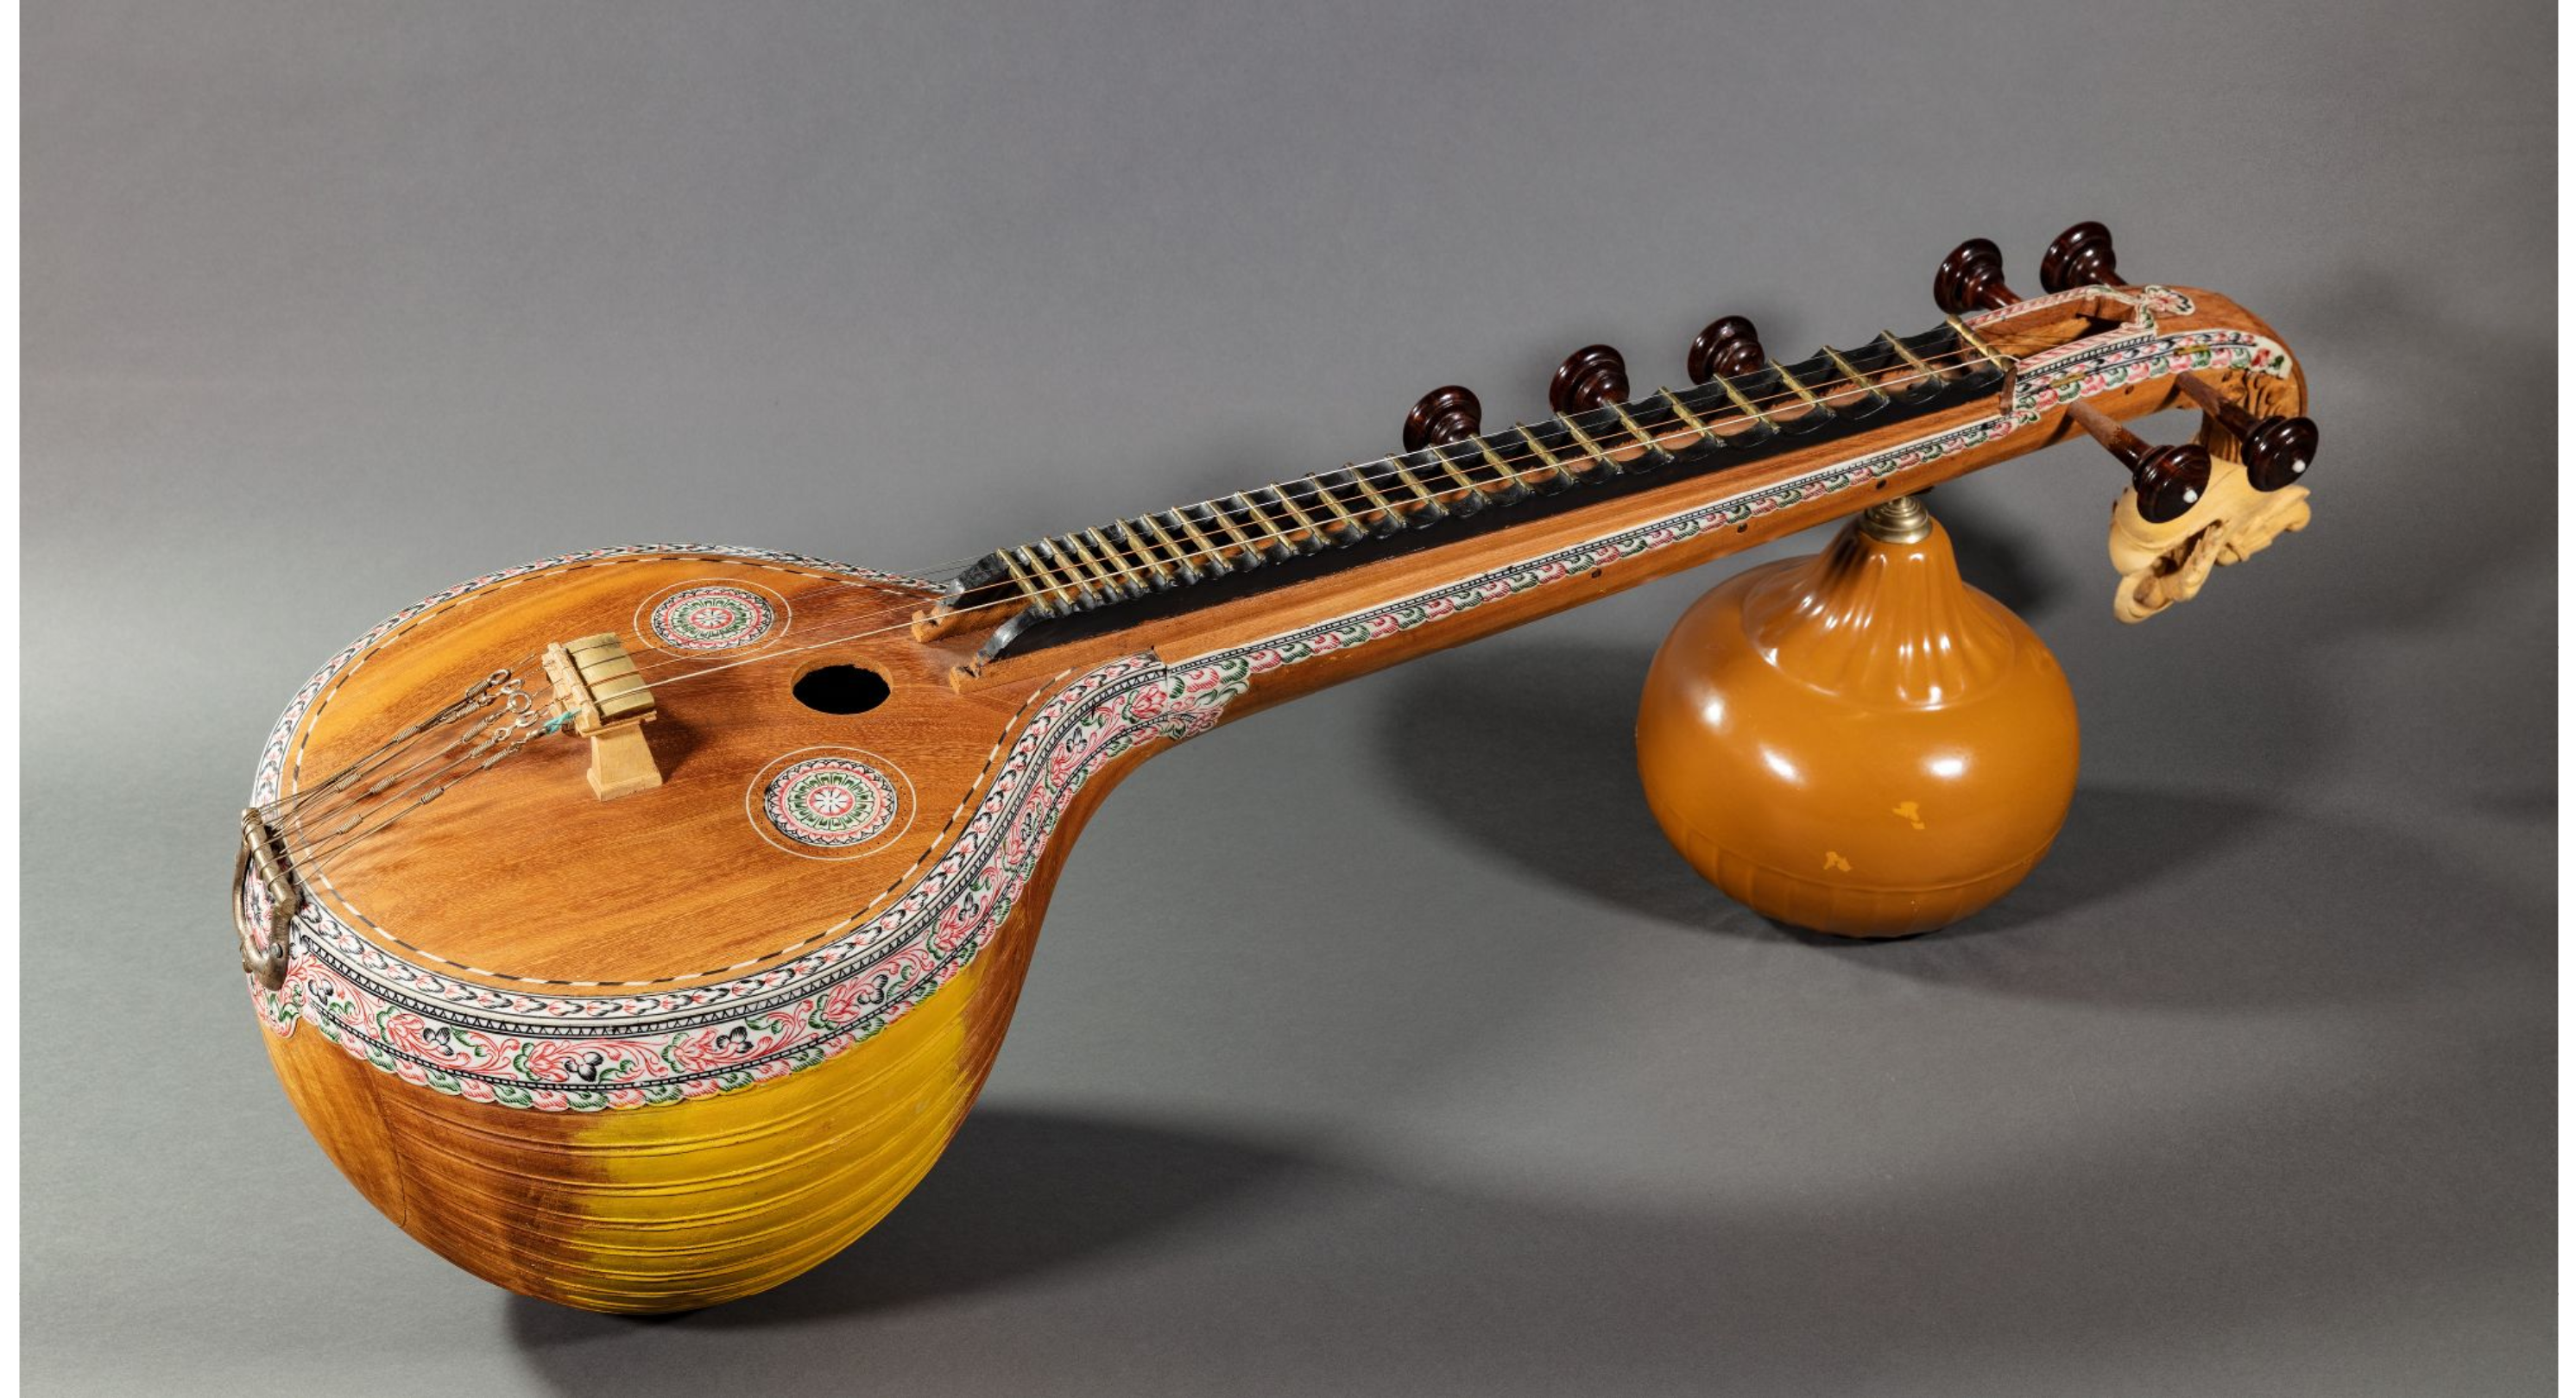
\includegraphics{veena}
  \caption{Veena from Chennai, Wikimedia Commons}
\end{marginfigure}
\begin{marginfigure}[-6\baselineskip]
  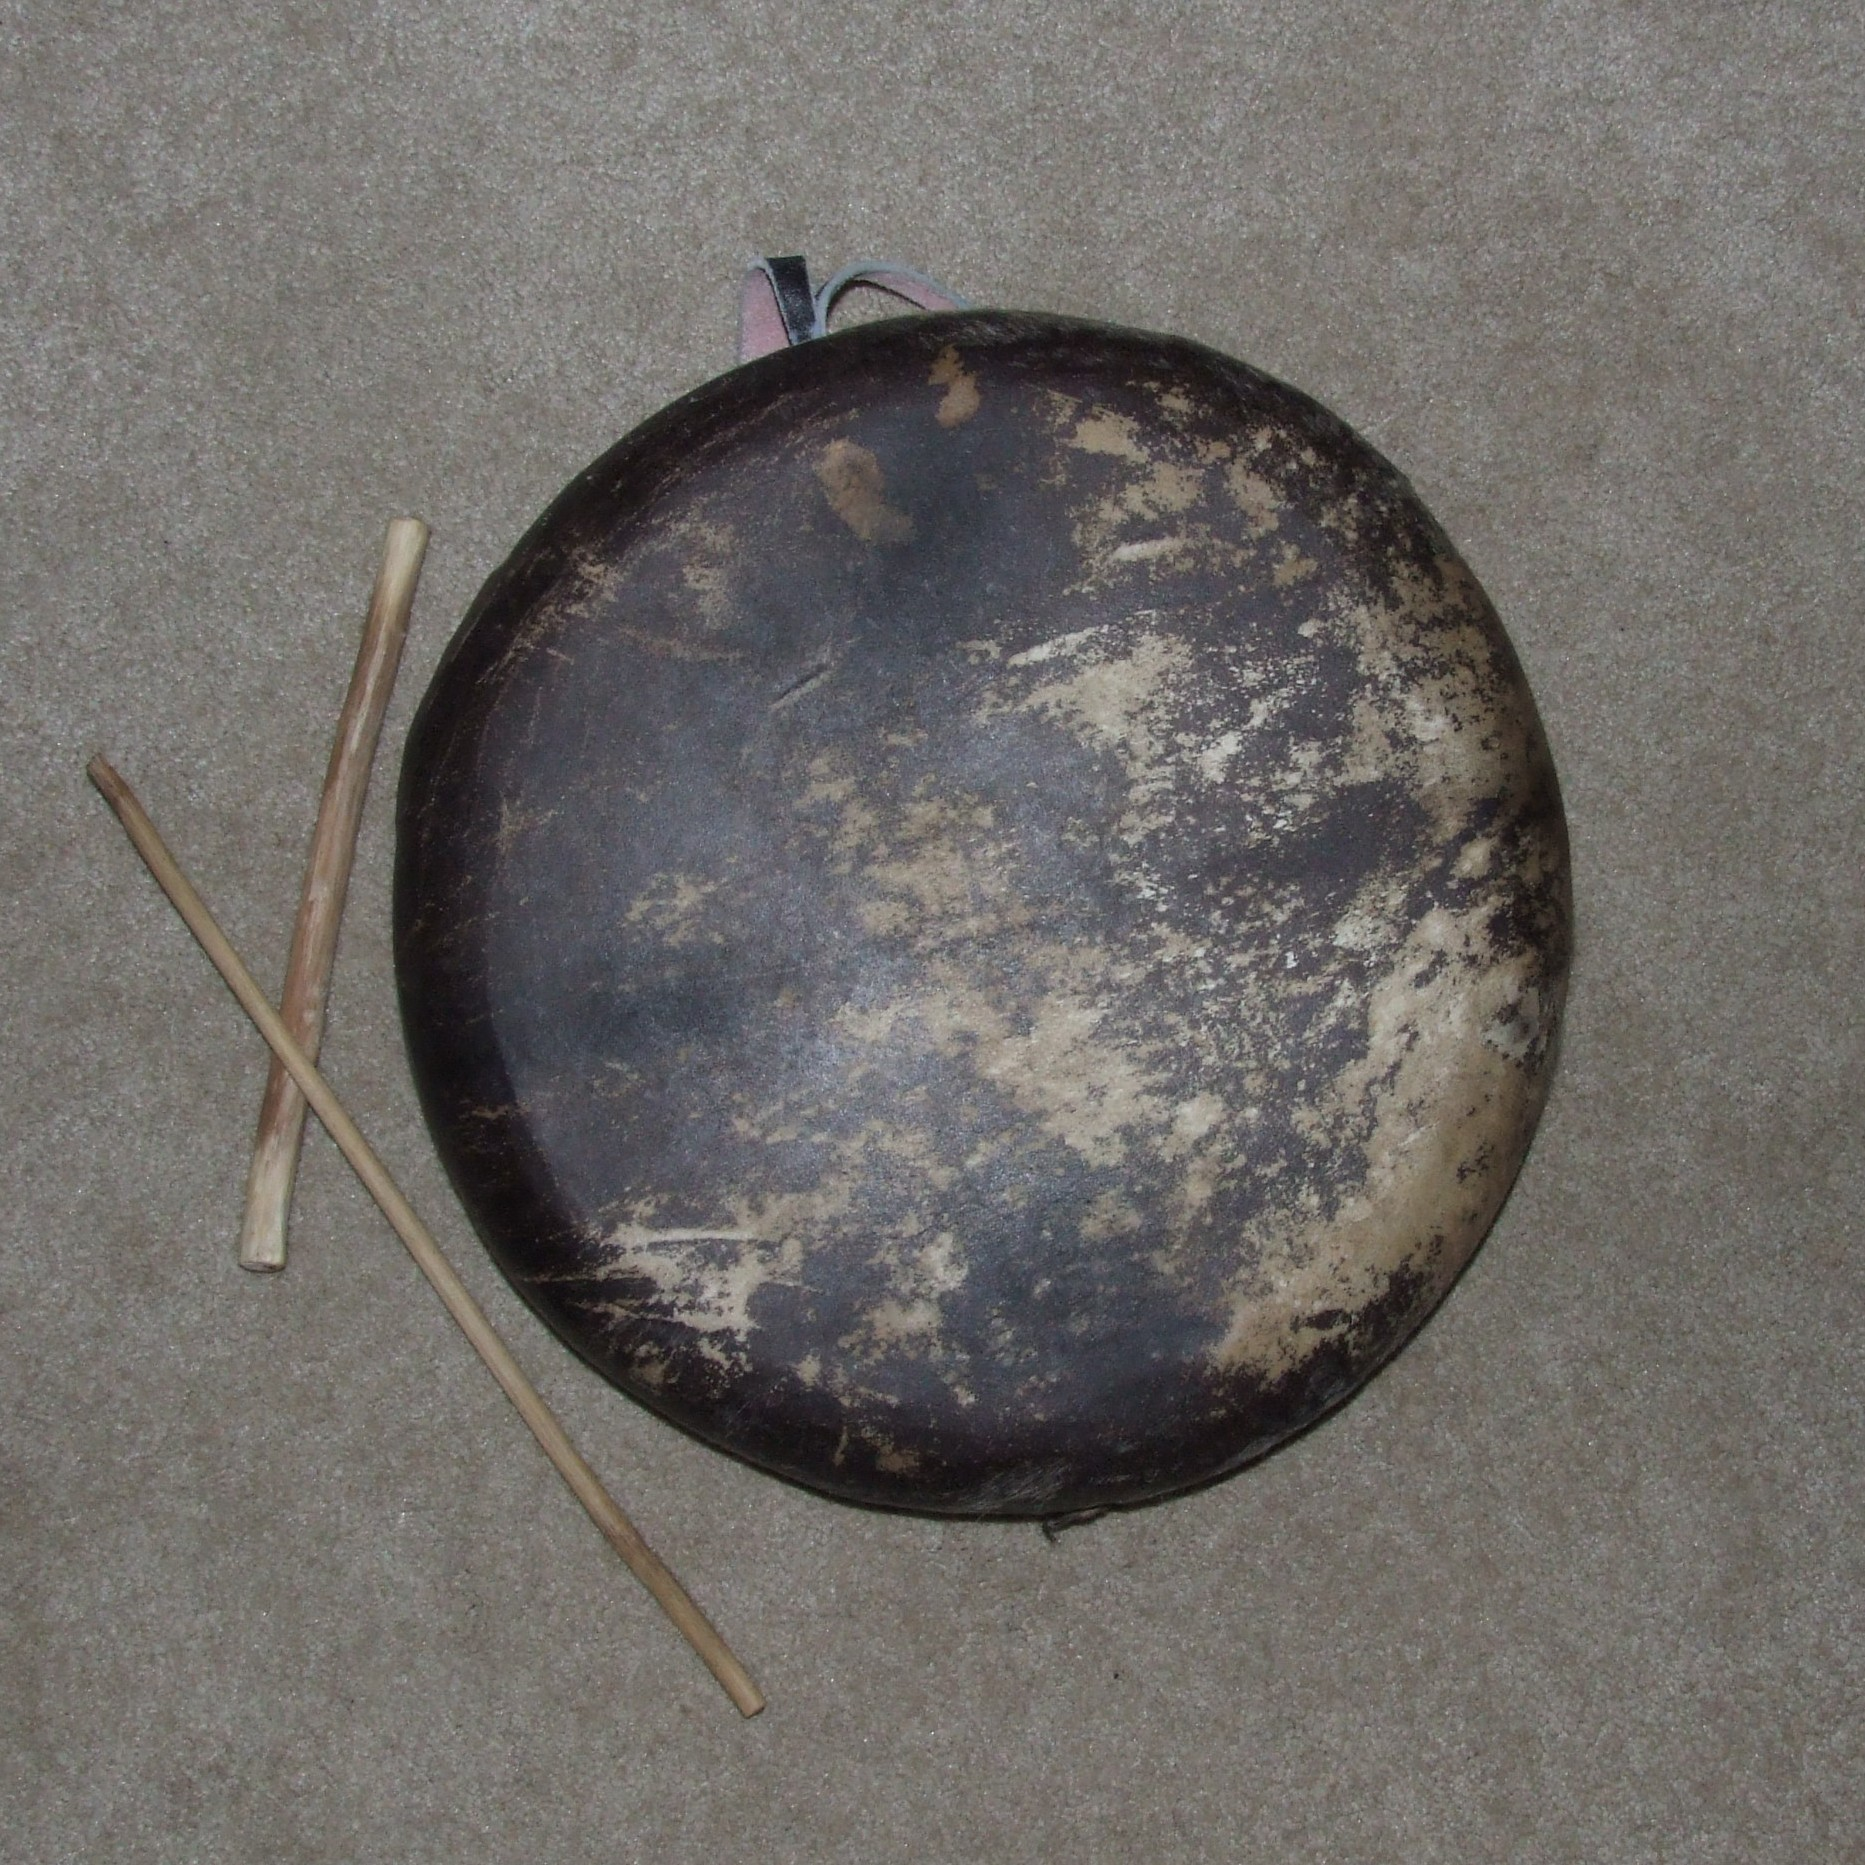
\includegraphics{parai}
\caption{Front side of a parai with the sticks used to play the instrument. Image by Prabhunkl, licensed under CC BY-SA 4.0}  
\end{marginfigure}
\begin{marginfigure}
  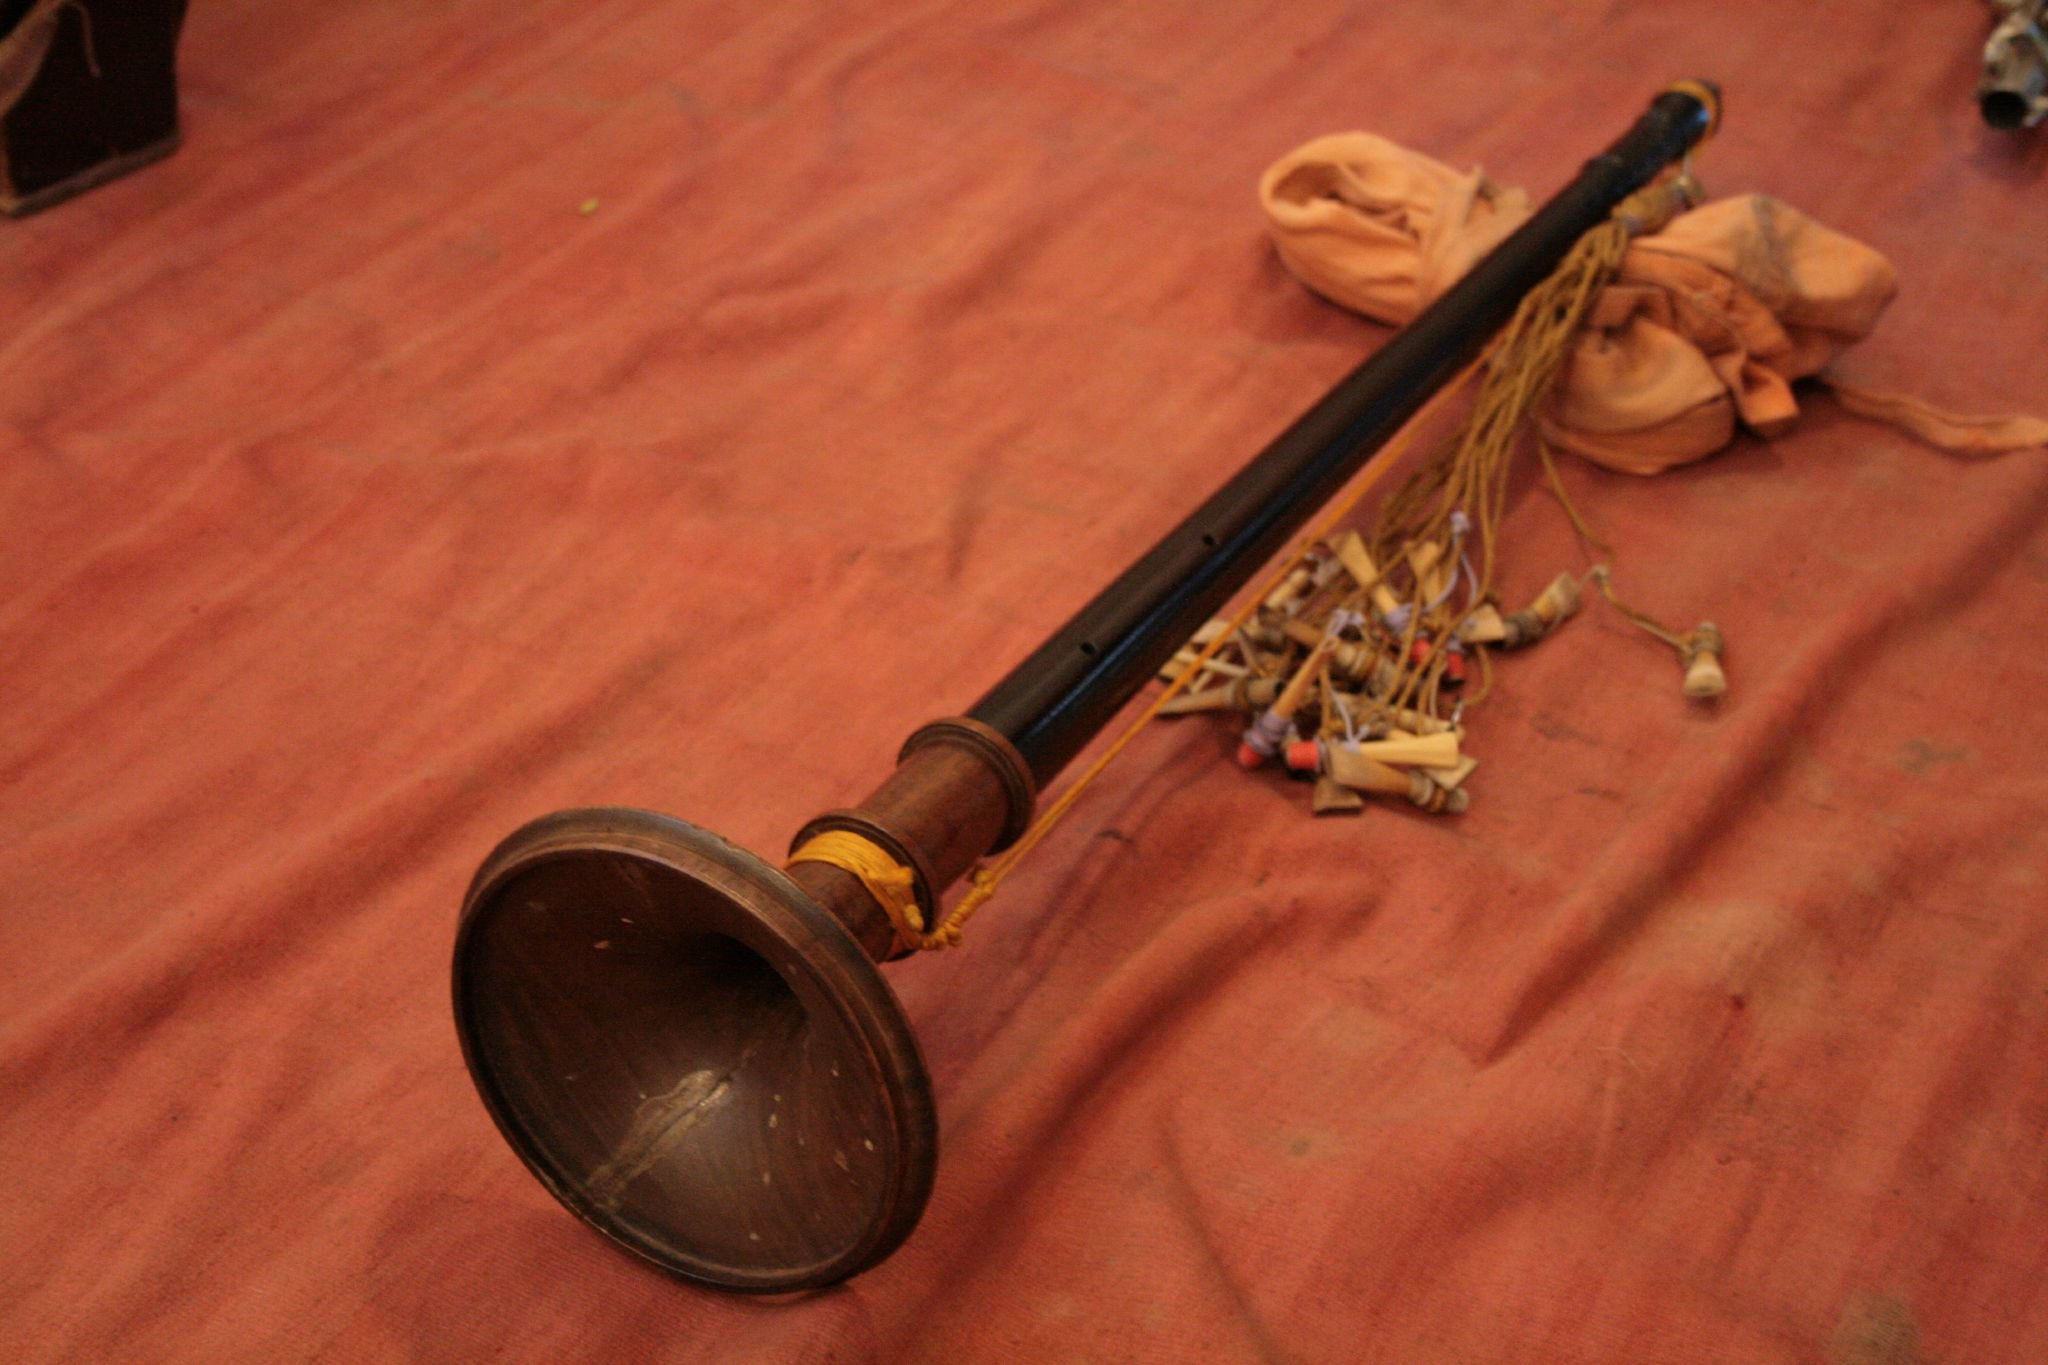
\includegraphics{nadaswaram}
\caption{Nadaswaram (also nagaswaram or nagasuram), Image by Ashwin Kamath}
\end{marginfigure}